The project is managed in seven phases. The implementation runs over six weeks, from 19 October to 29 November 2026, after the literature review and the stakeholder interview. Each phase depends on the one before it: the environment cannot be built before the scenarios are elicited, the scenario model is frozen before any agent is trained, and the experiments cannot run before the agents and baselines exist.

The seven phases group the eight research phases of Figure~\ref{fig:pipeline} for scheduling. Phase~1 covers specifying the problem; Phase~2, eliciting scenarios with the Directorate; Phase~3, both building and validating the environment and encoding the rules; Phase~4, both implementing the baselines and training the agents; Phase~5, running the experiments; and Phase~6, analysing the results. Phase~7, writing and submission, is not a research phase and so does not appear in Figure~\ref{fig:pipeline}.

\begin{center}\textbf{Project Timeline (19 October to 29 November 2026)}\end{center}

{\small
\begin{longtable}{|c|P{2.3cm}|P{4.8cm}|P{1.5cm}|P{1.6cm}|P{3.0cm}|}
\hline
\textbf{Phase} & \textbf{Phase Name} & \textbf{Key Activities} & \textbf{Weeks} & \textbf{Depends on} & \textbf{Deliverable} \\ \hline
\endfirsthead
\hline
\textbf{Phase} & \textbf{Phase Name} & \textbf{Key Activities} & \textbf{Weeks} & \textbf{Depends on} & \textbf{Deliverable} \\ \hline
\endhead
\multicolumn{6}{r}{\emph{Continued on next page}} \\
\endfoot
\endlastfoot
1 & Literature and Planning & Thematic literature review and Chapters 1--3; stakeholder interview with the Directorate (19 Oct); systematic literature review (23 Oct); approvals; elicitation workbook. & Before 19 Oct, Week 1 & -- & Proposal, systematic review, elicitation workbook. \\ \hline
2 & Scenario Elicitation & Elicitation session(s) with Directorate staff in the week of 26 October; scenario model of about 15 causes, about 10 symptoms, 20 checks and 10 rules written up as configuration files. & Week 2 & 1 & Scenario model v1. \\ \hline
3 & Environment and Rules & Incident generator and Gymnasium environment with the three ambiguity controls; the rules and the review-then-escalate mechanism; tests and leakage check; staff review of sample incidents; scenario model frozen at the end of the week. & Week 3 & 2 & Frozen scenario model; tested simulator and rule mechanism. \\ \hline
4 & Baselines and Training & Six baseline policies and the metrics module; pilot runs; small hyperparameter search; the agent, unconstrained and penalty-only agents and the PPO agent trained over ten seeds on the frozen model. & Week 4 & 3 & Baselines run end to end; trained agents. \\ \hline
5 & Experiments & Experiments 1--3 (baselines, effect of the mechanism, ablations); sensitivity to escalation cost; Experiment 4 (twelve ambiguity settings). & Week 5 & 4 & Results tables and charts. \\ \hline
6 & Analysis and Prototype & Confidence intervals, decision-mix charts and findings against the decision criteria for H1--H3; replay dashboard and results panel. & Weeks 5--6 & 5 & Findings summary; working prototype. \\ \hline
7 & Writing and Submission & Results chapter, revision of Chapters 1--3, poster, archive of code and configurations, presentation rehearsal. & Week 6 & 6 & Poster, report, archived code. \\ \hline
\end{longtable}
}

\begin{figure}[H]
\centering
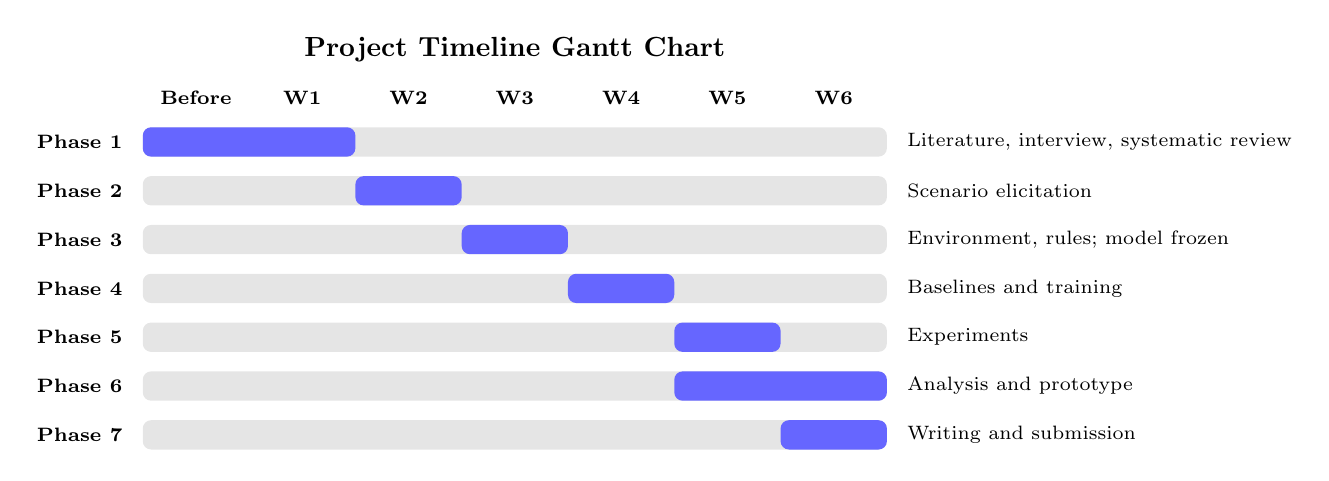
\begin{tikzpicture}[x=1.35cm,y=0.62cm]
\node[font=\bfseries] at (3.5,8.4) {Project Timeline Gantt Chart};
\foreach \w/\lab in {0/{Before},1/{W1},2/{W2},3/{W3},4/{W4},5/{W5},6/{W6}}
  \node[font=\scriptsize\bfseries] at (\w+0.5,7.4) {\lab};
\foreach \r/\lab/\s/\e/\d in {
  7/{Phase 1}/0/2/{Literature, interview, systematic review},
  6/{Phase 2}/2/3/{Scenario elicitation},
  5/{Phase 3}/3/4/{Environment, rules; model frozen},
  4/{Phase 4}/4/5/{Baselines and training},
  3/{Phase 5}/5/6/{Experiments},
  2/{Phase 6}/5/7/{Analysis and prototype},
  1/{Phase 7}/6/7/{Writing and submission}} {
  \node[font=\scriptsize\bfseries,anchor=east] at (-0.1,\r-0.5) {\lab};
  \fill[gray!20,rounded corners=3pt] (0,\r-0.8) rectangle (7,\r-0.2);
  \fill[blue!60,rounded corners=3pt] (\s,\r-0.8) rectangle (\e,\r-0.2);
  \node[font=\scriptsize,anchor=west] at (7.1,\r-0.5) {\d};
}
\end{tikzpicture}
\caption{Research project timeline Gantt chart. W1 begins on 19 October 2026 and W6 ends on 29 November 2026. The scenario model is frozen at the end of W3, before training begins in W4.}
\end{figure}
